\section{XML Build Tools}
Build systems are software tools designed to automate the process of program compilation.

\subsection{Apache Ant}
\subsubsection{What is it?/ What is it used for?}

Apache Ant is a software tool for automating software build processes, which uses XML to describe the build process and its dependencies.Please see figure~\ref{fig:buildxml}.

It was a replacement for the Unix make build tool. It is similar to Make but is implemented using the Java language, requires the Java platform, and is best suited to building Java projects.




\begin{figure}[hb]
    \center{}
    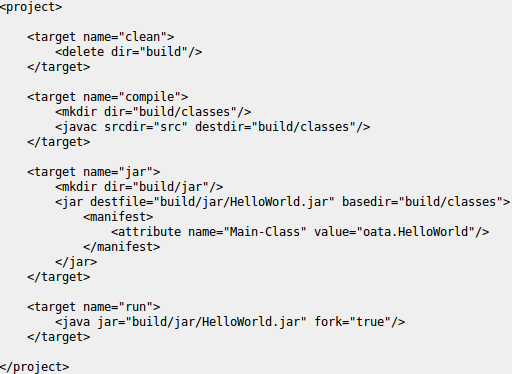
\includegraphics[width=1\textwidth]{buildxml}
    \caption{Ant build.xml file
    \protect\footnotemark}\label{fig:buildxml}
\end{figure}
\footnotetext{\url{https://ant.apache.org/manual/tutorial-HelloWorldWithAnt.html}}

\subsubsection{Why was it created?}



\begin{itemize}

\item Make-like tools are shell/OS dependant:These kind of programs are inherently shell-based: they evaluate a set of dependencies, then execute commands not unlike what you would issue on a shell. This means that you can easily extend these tools by using or writing any program for the OS that you are working on; however, this also means that you limit yourself to the OS, or at least the OS type, such as Unix, that you are working on.

\item Makefiles writing could be complicated

\end{itemize}


\subsubsection{Why is XML important?}

Instead of writing shell commands, the configuration files are XML-based, which gives the possibility of interpret the data more easily, and solve some of the portability issues forehead mentioned. This approach removes some of the expressive power that is inherent in being able to construct a shell command but gives the ability to be cross-platform. Another good thing about XML for creating build files is that it uses an ordered hierarchical structure. This structure fits well with build files, since the build steps mostly need to be executed in a specific order and steps can be grouped in multiple phases using the hierarchy.


\subsubsection{XML Related disadvantages}

Ant build files, which are written in XML, can be complex and verbose. The complex structure (hierarchical, partly ordered, and pervasively cross-linked) of Ant documents can be a barrier to learning. The build files of large or complex projects can become unmanageably large. Good design and modularization of build files can improve readability but not necessarily reduce size.

\subsection{Visual Build}
\subsubsection{What is it?/ What is it used for?}

It is a GUI program for Windows to automate building and deployment of desktop software, games and web applications, automating development and administrative tasks within an enterprise, and much more.
\subsubsection{Why was it created?}
Most existing build systems do not have a GUI available. There are a lot of people who like GUIs more than text files with commands, so this tool is a solution for those people.
\subsubsection{Why is XML important?}
The main reason for this build system to use XML is that it is text based. This means that it can easily be made a part of the source code repository. This way, even though it is not actually written by hand, the changes can still be seen using normal source control tools.

\subsection{Final Remarks}

XML has both advantages and disadvantages when using build systems.Please see table~\ref{table:advantages_disadvantages}. 

\begin{table}[hb]
    \begin{tabulary}{\textwidth}{cLL}
        \toprule
     \textbf{Aspect} & \textbf{ Advantages} & \textbf{ Disadvantages} \\
        \midrule
   \textbf{ Structure} & Easy to organize information & Can get very complex depending on the hierarchy \\
        \midrule
  \textbf{Text Based} & Useful for version control systems & Could be hard to read for humans \\
    \bottomrule
    \end{tabulary}
    \caption{Advantages vs. Disadvantages}\label{table:advantages_disadvantages}
\end{table}

Sources taken from~\autocites{wiki_apache_ant}{apacheorg_apache_ant}{kinook_visual_build}{wiki_visual_build}
